\chapter{Funktionalität}
\textcolor{red}{Funktionalität: Spezifikation der einzelnen Produktfunktionen mit genauer und detaillierter Beschreibung.}

Zur Entkopplung einzelner Module und leichteren Wartbarkeit verwendet die Anwendung eine Drei-Schichten Architektur bestehend aus Nutzeroberfläche, Business-Schicht und Daten-Schicht. 
\begin{figure}[H]
\begin{center}
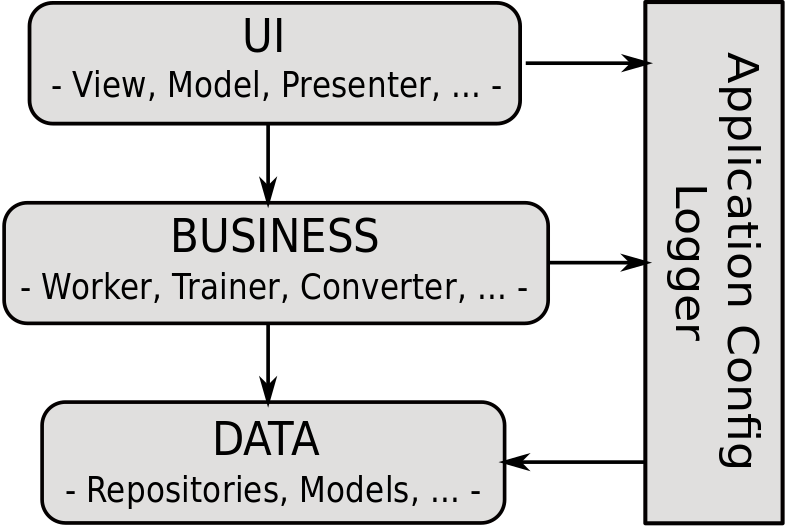
\includegraphics[width=10cm]{Abbildungen/UML/jan/SchichtenModell.png}
\end{center}
\end{figure}
Die Nutzeroberfläche dient der Nutzerinteraktion sowie der Darstellung der Eingabe- sowie verarbeiteten Daten. Sie implementiert dabei das MVP-Muster...

\textcolor{red}{ @Daniel: Hier bitte dein Part für das MVP-Pattern rein!!!}


In der Buisiness-Schicht werden alle fachspezifischen Verarbeitungen vorgenommen. Hierunter fallen beispielsweise die Vorwärtsberechnung sowie das Training eines künstlichen neuronalen Netzes oder die Konvertierung von Daten. Dazu werden für jede Entität spezifizsche Worker-Klassen bereitgestellt, die diese Aufgaben durchführen können.

\begin{figure}[H]
\begin{center}
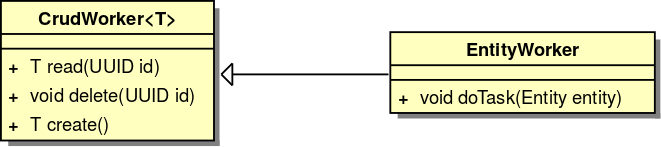
\includegraphics[width=10cm]{Abbildungen/UML/jan/workerClassDiagramm.png}
\end{center}
\end{figure}

Als unterste Schicht der Anwendung dient die Daten-Schicht der Persistierung von Daten. Hierfür stehen ihr diverse, von CRUD-Workern angesprochene Repositories zur Verfügung, die je nach Bedarf Daten (hier im Wesentlichen das Neuronale Netz) in eine Datenbank oder externe Dateien schreiben können.

In den nächsten Unterabschnitten folgt die ausführliche Beschreibung und geplante Umsetzung der von der Anwendung zu erbringenden Funktionalitäten.  

\section{Vorwärtsberechnung eines Neuronalen Netzes}

\begin{figure}[h]
\begin{center}
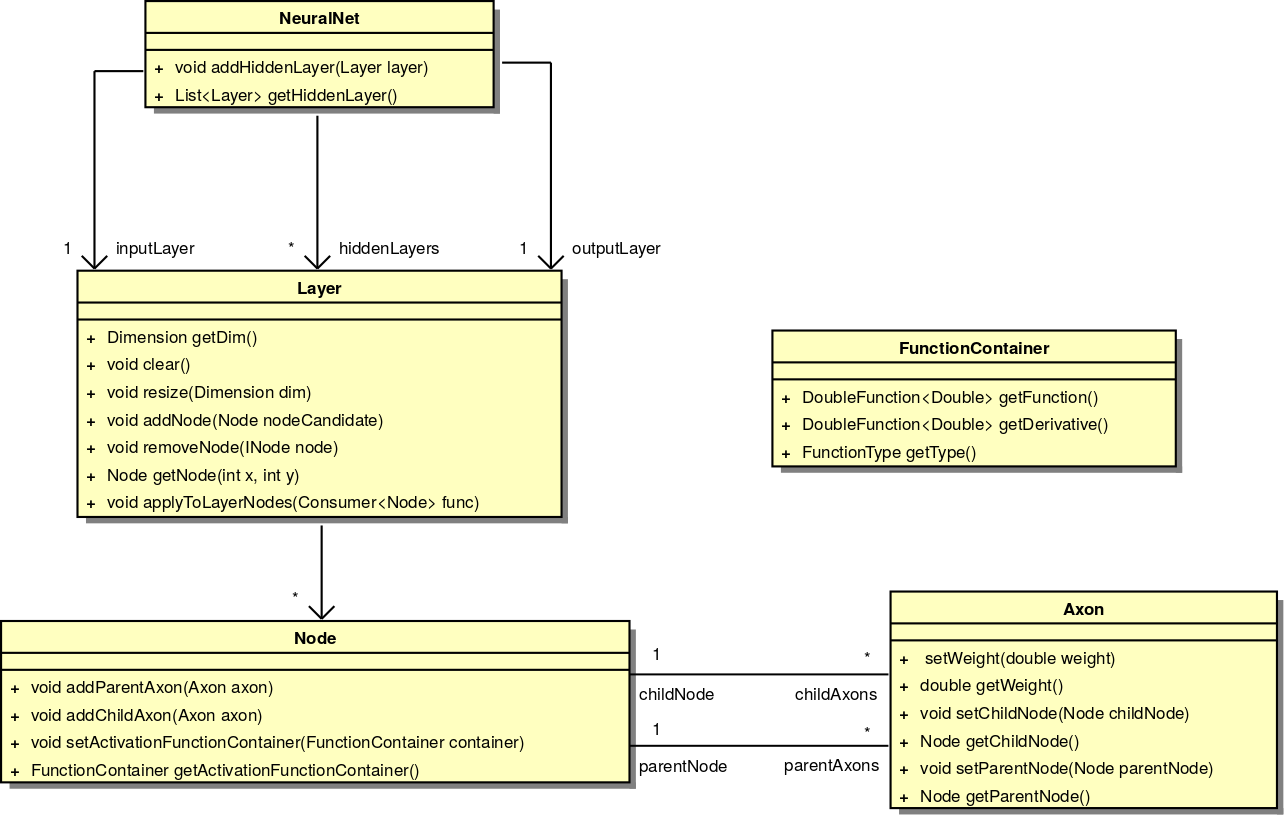
\includegraphics[width=\textwidth]{Abbildungen/UML/uml_ronny/neuralNetKlassenDiagramm.png}
\end{center}
\end{figure}


\begin{figure}[H]
\begin{center}
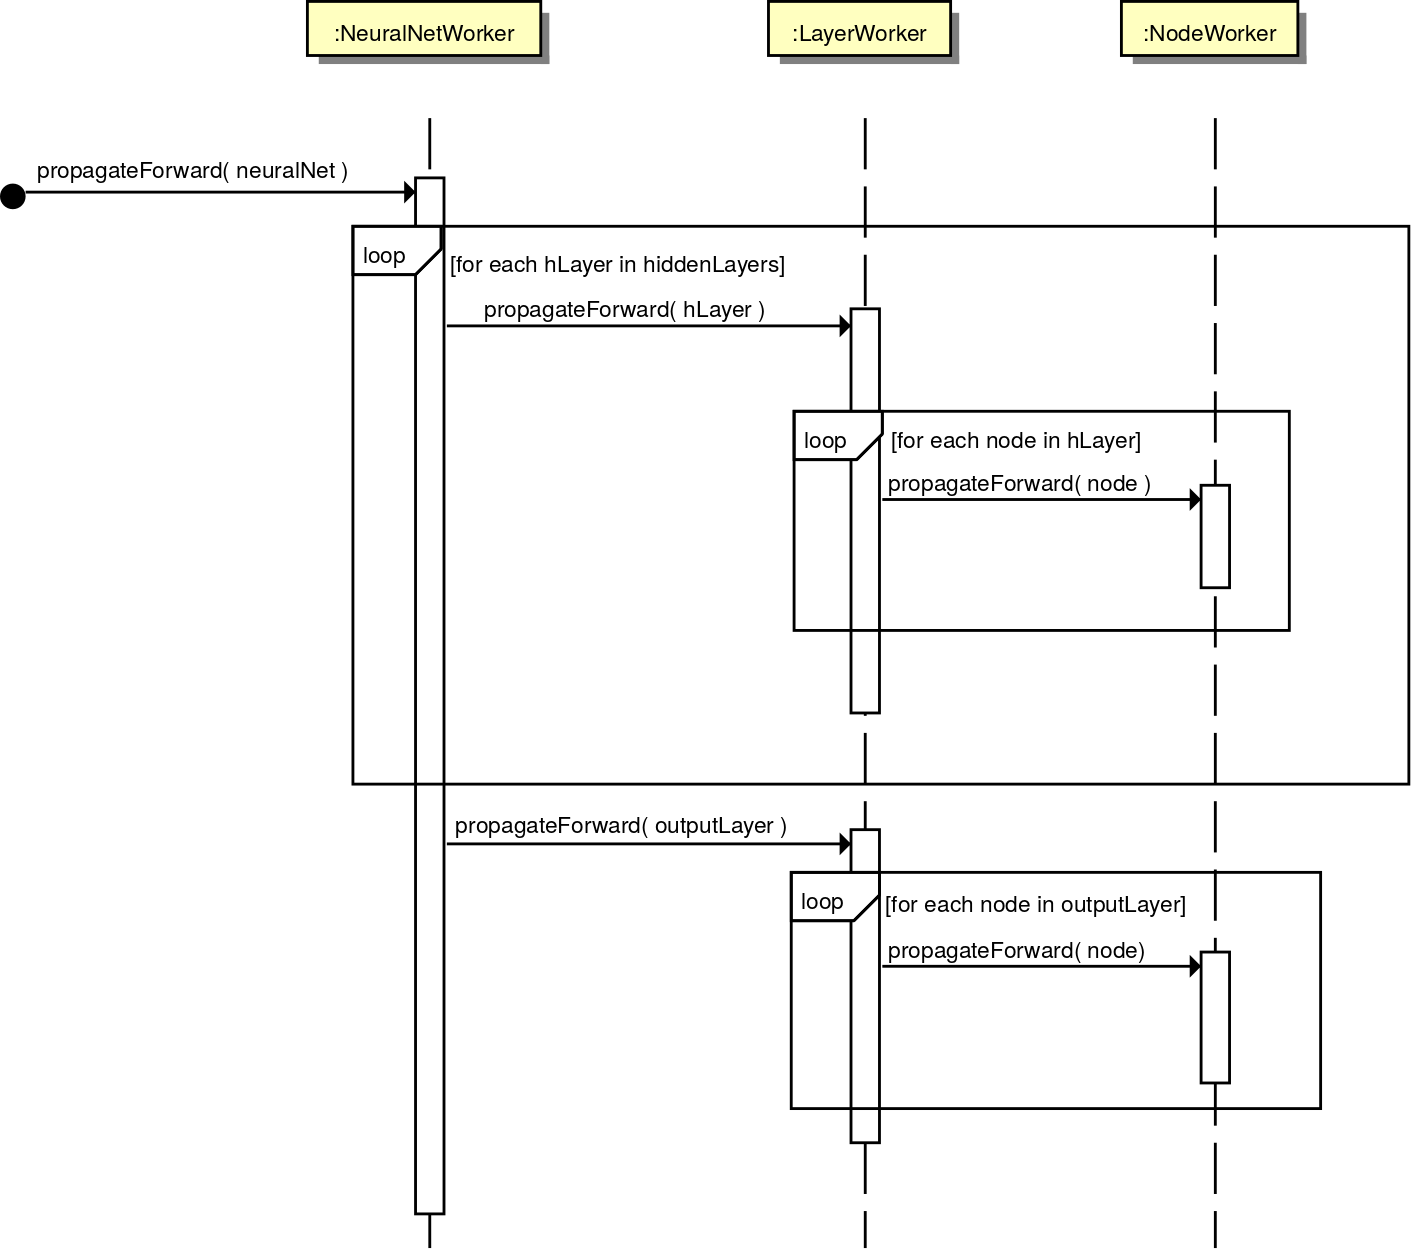
\includegraphics[width=13cm]{Abbildungen/UML/uml_ronny/forwardPropagationSD.png}
\end{center}
\end{figure}

\begin{figure}[H]
\begin{center}
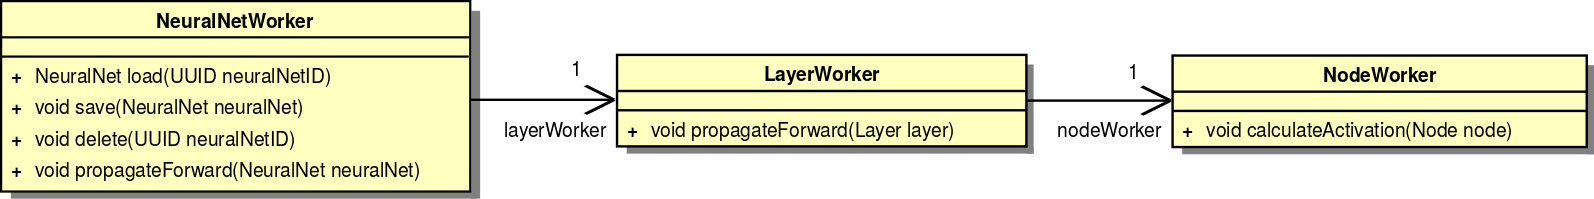
\includegraphics[width=\textwidth]{Abbildungen/UML/uml_ronny/workerKlassenDiagramm.png}
\end{center}
\end{figure}

\newpage
\section{Training eines Neuronalen Netzes}

Das Training eines Neuronalen Netzes erfolgt mit Hilfe des Gradienten-Abstieg-Algorithmus. Durch den Vergleich von tatsächlicher Netzwerkausgabe zur erwarteten Ausgabe werden dabei beginnend beim Ausgabelayer sukzessive Anpassungen an den Netzwerkknoten und Netzwerkaxon vorgenommen. Für jede Abstraktionstufe des Neuronalen Netzes wird dabei ein eigener Trainer angelegt, der für die Rückwärtspropagierung des Ausgabefehlers zuständig ist.\\[-0.5cm]
\begin{figure}[H]
\begin{center}
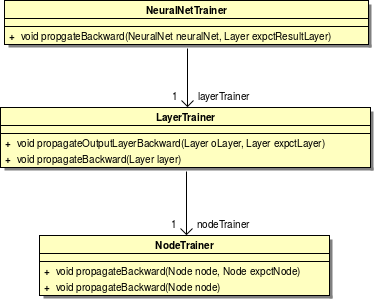
\includegraphics[width=10cm]{Abbildungen/UML/jan/classdiagrammTraining.png}
\caption{Klassendiagramm der Trainingsworker für das Neuronale Netz, Layer und Nodes.}
\label{fig_cdTraining}
\end{center}
\end{figure}
\vspace{-0.4cm}
Der Ablauf eines Trainingdurchlaufs stellt sich als Sequenzdiagramm wie folgt dar:
\begin{figure}[H]
\begin{center}
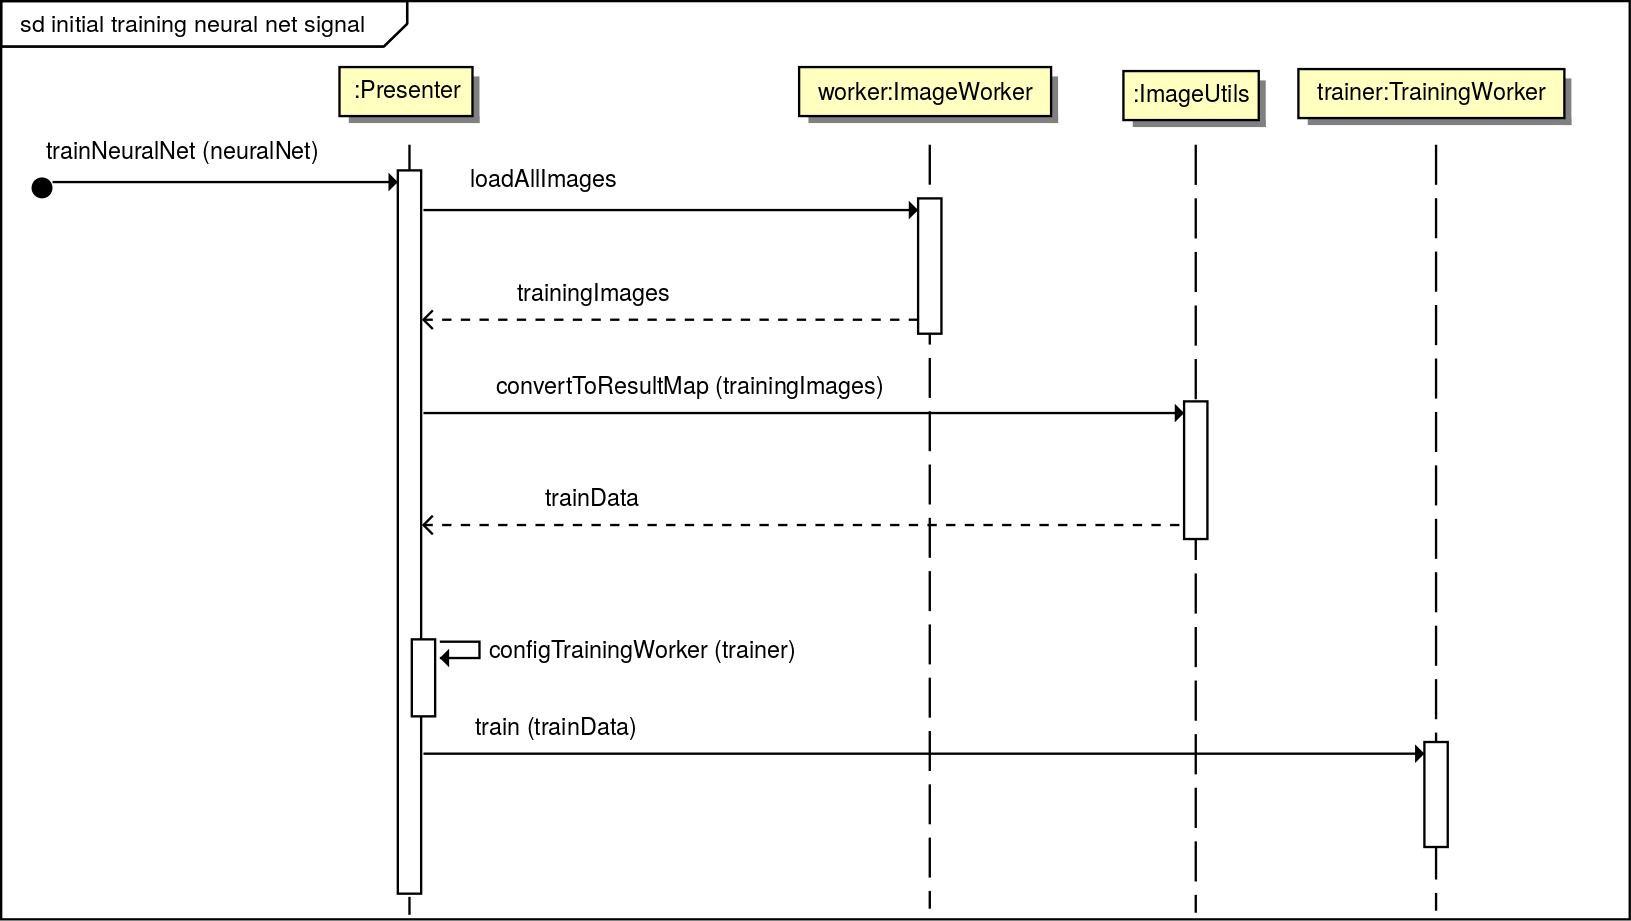
\includegraphics[width=14.2cm]{Abbildungen/UML/jan/trainNeuralNet.png}
\caption{Sequenzdiagramm zum Trainingsprozess beginnend am Presenter.}
\label{fig_sdTraining}
\end{center}
\end{figure}
\begin{figure}[H]
\begin{center}
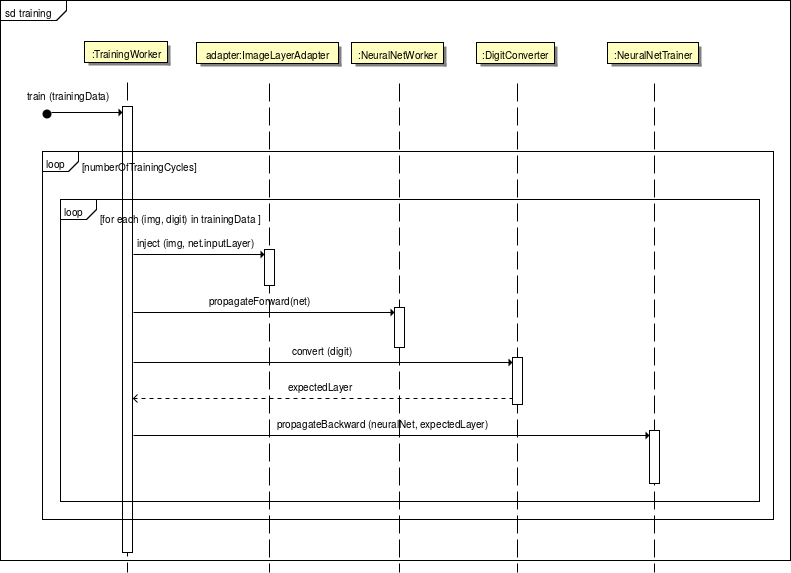
\includegraphics[width=14.2cm]{Abbildungen/UML/jan/trainDetailed1.png}
\caption{Sequenzdiagramm für Trainingsprozess im Trainingsworker.}
\label{fig_sdTraining}
\end{center}
\end{figure}
\vspace{-0.5cm}
\begin{figure}[H]
\begin{center}
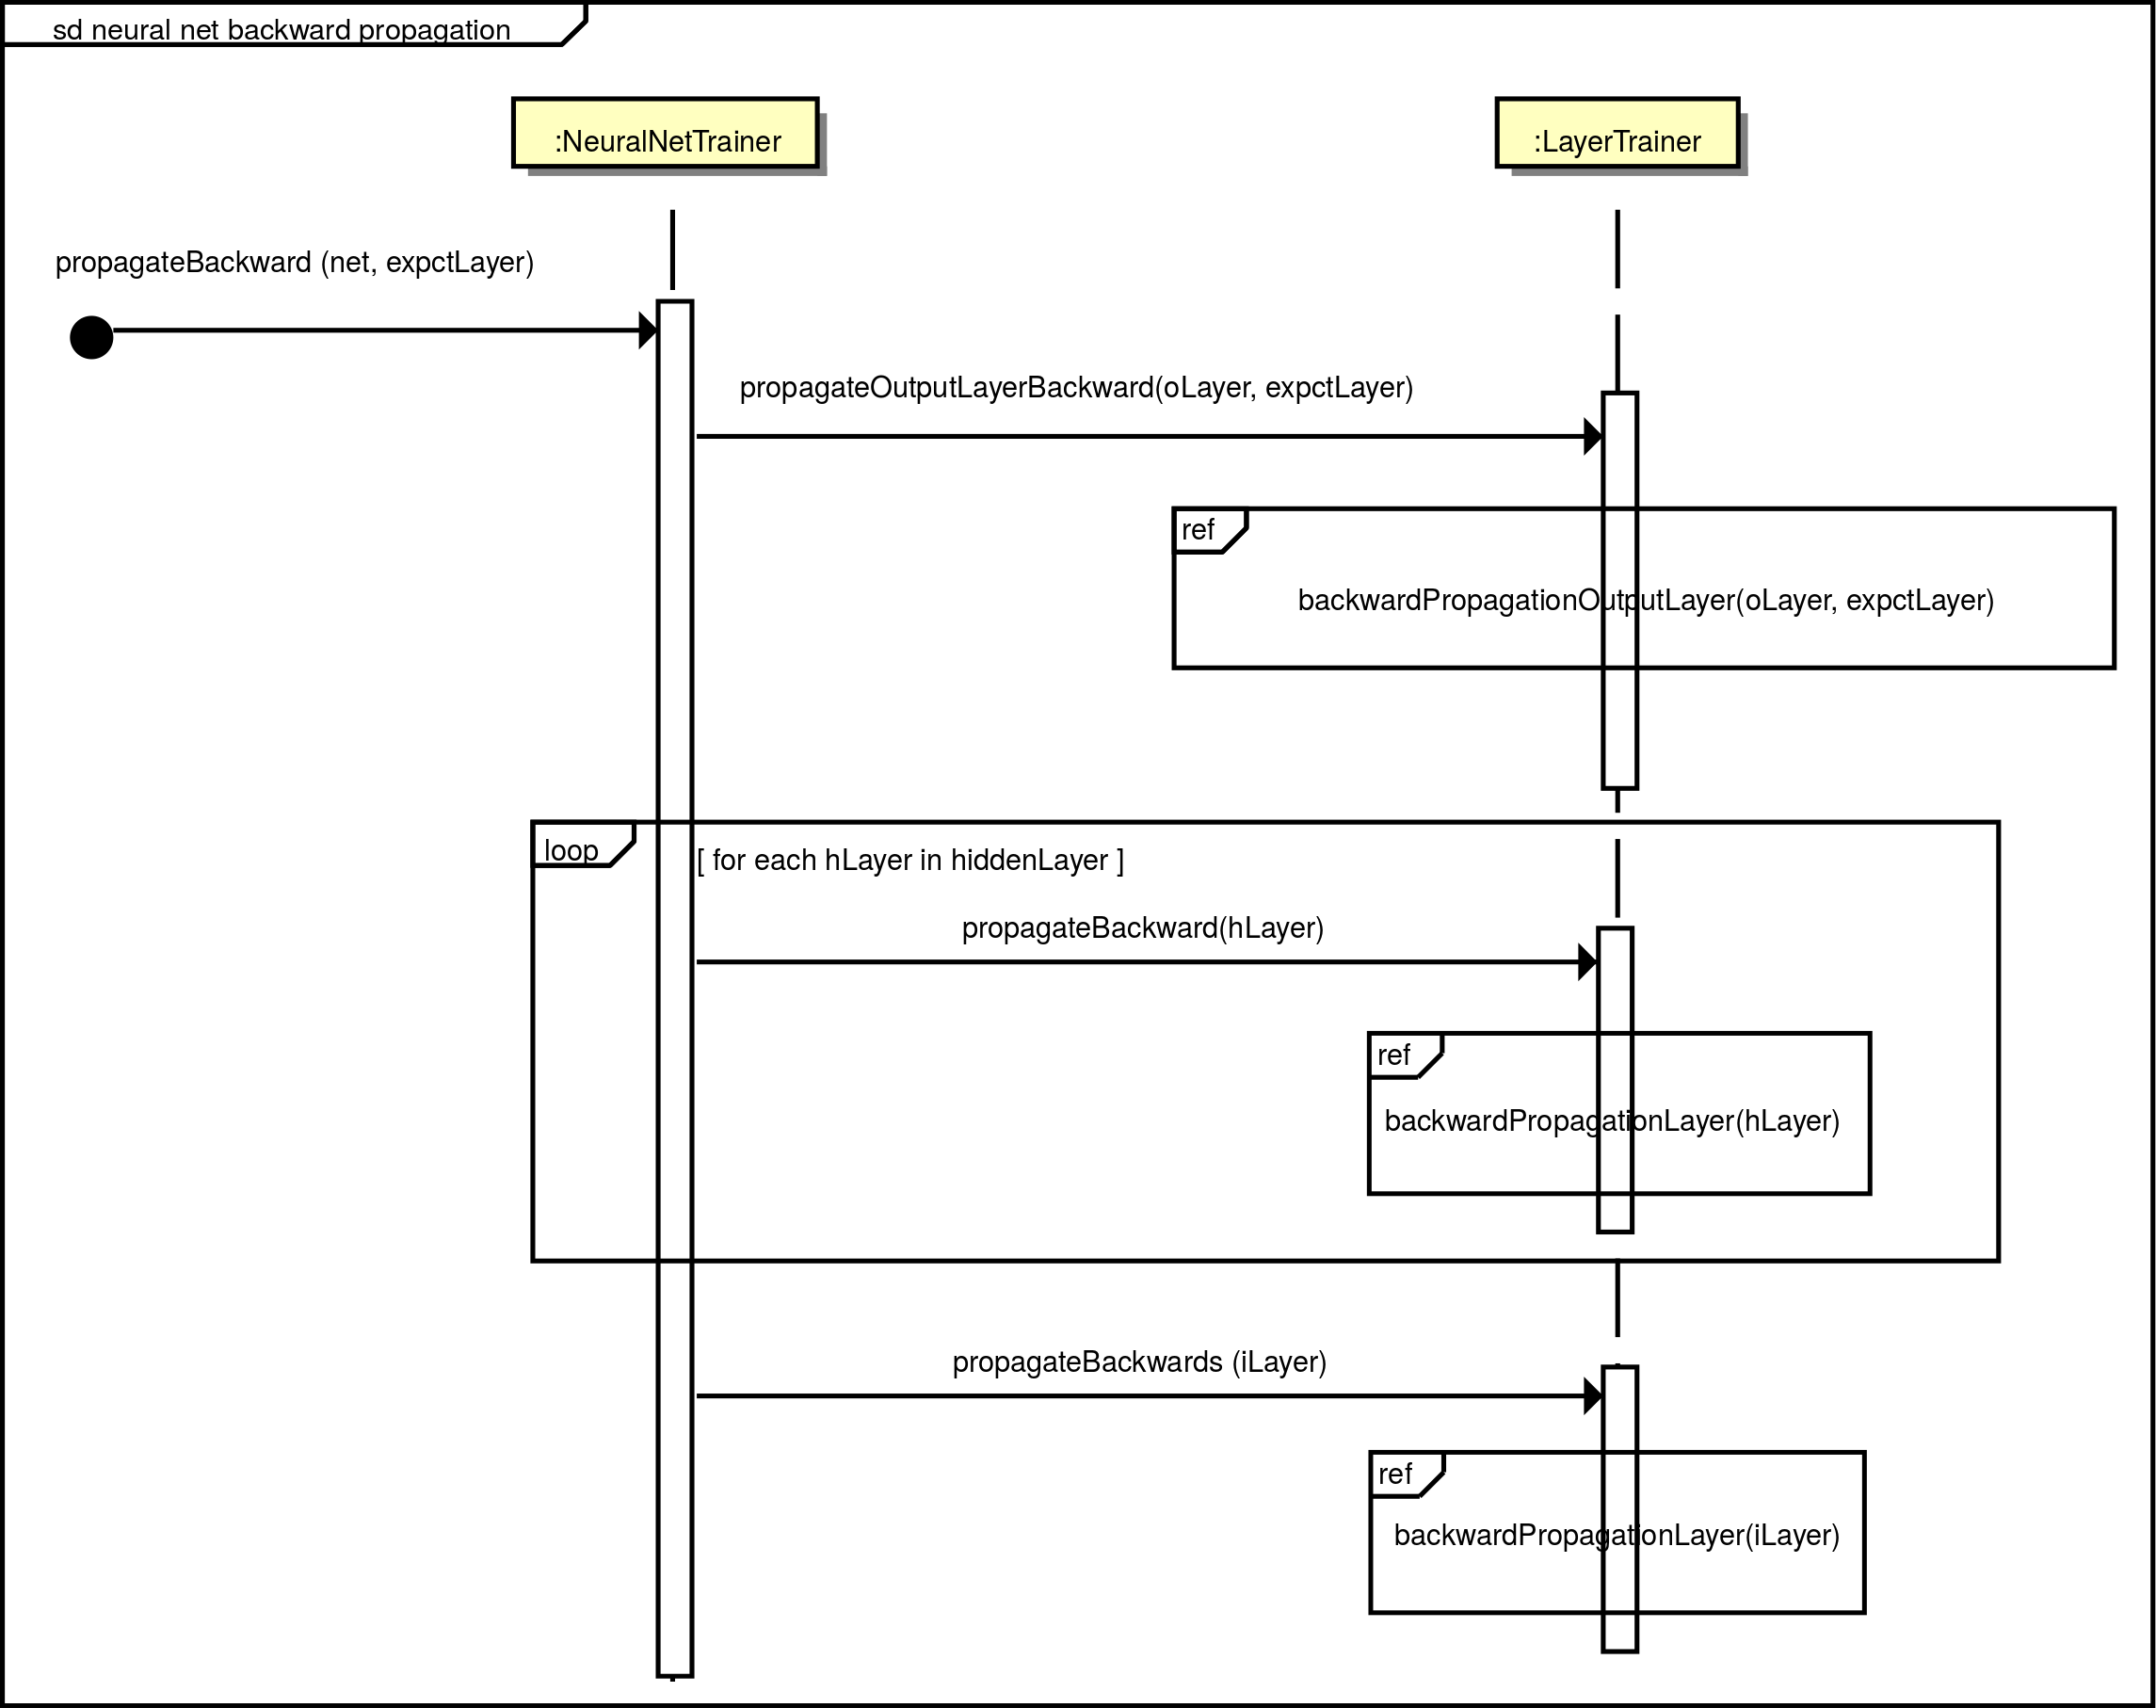
\includegraphics[width=14.2cm]{Abbildungen/UML/jan/gradientdescent1.png}
\caption{Sequenzdiagramm zur Backpropagation beginnend beim Neuronalen Netz.}
\label{fig_sdBackpropagation}
\end{center}
\end{figure}
